\documentclass[tikz,border=5pt]{standalone}

\usetikzlibrary{calc}

\newcommand
    {\XOR}
    {%
        \oplus%
    }

\begin{document}
    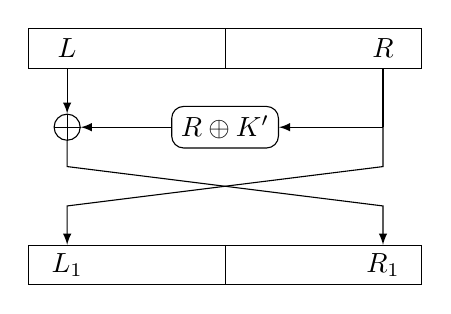
\begin{tikzpicture}
        % 1. Function F_k1
        \node (f1) at (0,-1.5cm) [minimum width=1cm,rounded corners=1ex,draw] {$R \XOR K'$};

        % 2. Top Block (L0, R0)
        \node (p0) at (0, -0.5cm) [minimum width=5cm,minimum height=0.5cm,draw] {};
        \draw[-] (p0.north) -- (p0.south);
        
        % Accurately center L0 and R0 within the two halves using the calc library
        \node (l0) at ($(p0.west)!0.2!(p0.center)$) {$L$};
        \node (r0) at ($(p0.center)!0.8!(p0.east)$) {$R$};

        % Align XOR perfectly under L0, and horizontally with f1
        \node (xor1) [circle, draw] at (l0 |- f1) {};
        \draw[-] (xor1.north) -- (xor1.south);
        \draw[-] (xor1.east) -- (xor1.west);
        \draw[-latex] (f1.west) -- (xor1.east);

        % Connections from Top Block
        \draw[-latex] (l0 |- p0.south) -- (xor1.north); 
        
        % Right vertical wire drops from R0 down to f1's horizontal level
        \draw[-] (r0 |- p0.south) -- (r0 |- f1.east);

        % 3. Bottom Block (L1, R1)
        \node (p1) at (0, -3.25cm) [minimum width=5cm,minimum height=0.5cm,draw] {}; 
        \draw[-] (p1.north) -- (p1.south);
        
        \node (l1) at ($(p1.west)!0.2!(p1.center)$) {$L_1$};
        \node (r1) at ($(p1.center)!0.8!(p1.east)$) {$R_1$};

        % 4. Cross-wiring 
        % Branch right wire into f1
        \draw[-latex] (r0 |- f1.east) -- (f1.east);
        
        % Define precise Y-coordinates for the crossing so it forms a perfect "X"
        \coordinate (CrossTop) at (0, -2.0cm);
        \coordinate (CrossBot) at (0, -2.5cm);
        
        % Right side to Left side (R0 -> L1)
        \draw[-latex] (r0 |- f1.east) -- (r0 |- CrossTop) -- (l0 |- CrossBot) -- (l1 |- p1.north);
        
        % Left side to Right side (L0/XOR -> R1)
        \draw[-latex] (xor1.south) -- (l0 |- CrossTop) -- (r0 |- CrossBot) -- (r1 |- p1.north);
        
    \end{tikzpicture}
\end{document}